\documentclass[a4paper]{article}
\usepackage[english]{babel}
\usepackage[utf8x]{inputenc}
\usepackage[T1]{fontenc}
\usepackage{listings}
\usepackage[a4paper,top=2cm,bottom=2cm,left=2cm,right=2cm,marginparwidth=1.75cm]{geometry}
\usepackage{amsmath}
\usepackage{graphicx}
\usepackage[colorinlistoftodos]{todonotes}
\usepackage[colorlinks=true, allcolors=blue]{hyperref}
\usepackage{wasysym} % smileys
\setlength\parindent{0pt} % indent

% my commands:
\newcommand{\n}{\newline}
\newcommand{\tab}{\hspace{1cm}}

\begin{document}
\text{}\vspace{-0.1cm}
{\fontfamily{pbk}\fontsize{12}{15}\selectfont \hspace{-0.5cm}\text{10. domácí úkol | Vilém Zouhar}}

\section{Funkce dvou proměnných}
\subsection{Definiční obor}
\begin{align*}
	& \bigg| \frac{x}{x+y} \bigg| \le 1 \Rightarrow \frac{x}{x+y} \le 1 \wedge -1 \le \frac{x}{x+y} \Rightarrow \\
	& x+y > 0 (\Rightarrow x > -y) & x+y < 0 (\Rightarrow x < -y) \\
	& x \le x+y \wedge -x-y \le x & x \ge x+y \wedge -x-y \ge x \\
	& 0 \le y \wedge -y \le 2x & 0 \ge y \wedge -y \ge x \\
	& 0 \le y \wedge -y \le 2x \wedge  x > -y & 0 \ge y \wedge -y \ge x \wedge x < -y \\
	&& \\
	& \Rightarrow & (x > 0 \wedge y > 0) \\
	&& \vee \tab \hspace{0.48cm} (x < 0 \wedge y < 0) \\
	&& \vee \tab (x > 0 \wedge y < -2x) \\
	&& \vee \tab (x < 0 \wedge y > -2x) \\
	&& \vee \tab [(x = 0 \vee x = 0) \wedge (x \ne 0 \vee y \ne 0)] \\
	&& (\text{osy kromě počátku}) \\
%	&& \text{v počátku lze spojitě dodefinovat hodnotou 1}
\end{align*}

\vspace{-2.4cm}\hspace*{2.2cm}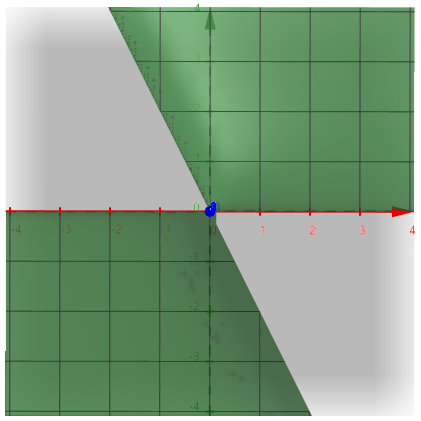
\includegraphics[width=3cm]{double_fun}

\subsection{Gradient}

\begin{align*}
	& \frac{\partial f}{\partial x} (x,y) = \frac{-\frac{x+y-x}{(x+y)^2}}{\sqrt{1-\big(\frac{x}{x+y}\big)^2}}	= \frac{-y}{|x+y|\sqrt{(x+y)^2 - x^2}}, \tab x \ne -y \\
	& \frac{\partial f}{\partial y} (x,y) = \frac{\frac{x}{(x+y)^2}}{\sqrt{1-\big(\frac{x}{x+y}\big)^2}} = \frac{x}{|x+y|\sqrt{(x+y)^2-x^2}}, \tab x \ne -y \\
	& \Rightarrow \nabla f \text{v bodě $(1,1)$} = \bigg(\frac{-1}{2\sqrt{3}}, \frac{1}{2\sqrt{3}}\bigg)
\end{align*}

\subsection{Totální diferenciál}

Paricální derivace jsou v okolí bodu $(1,1)$ spojité, tedy funkce je v tomto bodě diferencovatelná.
\begin{align*}
	& Df_{(1,1)}(x,y) = \frac{-1}{2\sqrt{3}} ( x - 1) + \frac{1}{2\sqrt{3}} ( y - 1) + f(1,1) = \frac{-1}{2\sqrt{3}} ( x - 1) + \frac{1}{2\sqrt{3}} ( y - 1) + \frac{\pi}{3}
\end{align*}

\subsection{Aproximace}
\begin{align*}
	& Df_{(1,1)}(1.04, 0.99) \approx 1.03
\end{align*}

\pagebreak
\section{Anuloid}

\subsection{Popis}
\begin{align*}
		& t = \sqrt{8 \sqrt{x^2 + y^2}-x^2 - y^2 - 12},\tab r = -\sqrt{8 \sqrt{x^2 + y^2}-x^2 - y^2 - 12} \\
		& A = t \cup r
\end{align*}
 
\subsection{Tečná rovina}
Jelikož je třetí souřadnice kladná, zajímá nás funkce $t$ v bodě $(0,3)$. Pro výpočet tečné roviny první určíme gradient této funkce a z toho vypočítáme totální diferenciál.

\begin{align*}
	 & \frac{\partial t}{\partial x} (x,y) = - \frac{x}{\sqrt{-12 - x^2 - y^2 + 8 \sqrt{x^2 + y^2}}} + \frac{4x}{\sqrt{x^2 + y^2} \sqrt{-12 - x^2 - y^2 + 8 \sqrt{x^2 + y^2}}} \\
	 & \frac{\partial t}{\partial y} (x,y) = \frac{-2 y + \frac{8 y}{\sqrt{x^2 + y^2}}}{2 \sqrt{-12 - x^2 - y^2 + 8 \sqrt{x^2 + y^2}}}
\end{align*}
Parciální derivace jsou v okolí $(0,3)$ spojité, tedy můžeme vypočítat totální diferenciál.
\begin{align*}
	& Dt_{(0,3)}(x,y) = \frac{\partial t}{\partial x} (0, 3) x + \frac{\partial t}{\partial y} (0,3) (y-3) + t(0,3) \\
	& = \frac{y-3}{\sqrt{3}} + \sqrt{3}\\
	& \Rightarrow \text{pokud jsme neudělali chybu v ověření spojitosti paricálních derivací, pak tečná rovina existuje.}
\end{align*}

\section{Podíl souřadnic}

\subsection{Gradient}
\begin{align*}
	& \frac{\partial f}{\partial x} (x,y) = \frac{1}{y}; \tab \frac{\partial f}{\partial y} (x,y) = \frac{-x}{y^2} \\
	& \nabla f = \bigg(\frac{1}{y}, \frac{-x}{y^2}\bigg), y \ne 0 \\
	& \text{gradient spojitý kromě y souřadnicové osy}
\end{align*}
\subsection{Totální diferenciál}
\begin{align*}
	Df_{(a,b)}(x,y) = \frac{x-a}{b} + \frac{-a(y-b)}{b^2} + \frac{a}{b}, y \ne 0
\end{align*}
\end{document}
